\documentclass[aspectratio=169,11pt,t]{beamer}

% ---------- Style: matches the Week 1 proposal (navy, Palatino body, Helvetica labels) ----------
\usepackage[T1]{fontenc}
\usepackage{mathpazo}
\usepackage{helvet}
\usepackage{graphicx}

\definecolor{navy}{HTML}{1F3864}
\definecolor{midgray}{HTML}{595959}
\definecolor{hairline}{HTML}{C8C8C8}

\setbeamertemplate{navigation symbols}{}
\setbeamertemplate{itemize items}{\textcolor{navy}{\footnotesize\textbullet}}
\setbeamercolor{normal text}{fg=black}
\setbeamercolor{structure}{fg=navy}
\setbeamerfont{normal text}{family=\rmfamily}
\usefonttheme{serif}

% footer: matches proposal footer register
\setbeamertemplate{footline}{%
  \hspace{0.45cm}{\sffamily\fontsize{6.5}{8}\selectfont\color{midgray}ENNACIRI \textbar\ EARLY-WARNING MODEL FOR U.S. BANK CAPITAL DISTRESS \textbar\ JULY 2026}%
  \hfill{\sffamily\fontsize{6.5}{8}\selectfont\color{midgray}\insertframenumber\ OF \inserttotalframenumber}\hspace{0.45cm}\vspace{0.25cm}}

% section-label style headline like the proposal
\newcommand{\slidelabel}[1]{%
  {\sffamily\bfseries\fontsize{10}{13}\selectfont\color{navy}\MakeUppercase{#1}}\par
  \vspace{-6pt}\textcolor{hairline}{\rule{\textwidth}{0.5pt}}\par\vspace{8pt}}

\begin{document}

% ---------- Slide 1: Title ----------
\begin{frame}
  \vspace{52pt}
  {\sffamily\fontsize{8}{11}\selectfont\color{midgray}MSDS 696 DATA SCIENCE PRACTICUM II \quad\textbar\quad WEEK 1 PRACTICE TALK}\par\vspace{12pt}
  {\sffamily\bfseries\fontsize{25}{30}\selectfont\color{navy}Early-Warning Model for\\[2pt]U.S. Bank Capital Distress}\par\vspace{9pt}
  {\fontsize{12.5}{17}\selectfont\itshape\color{midgray}Identifying banks at risk of becoming undercapitalized\\while corrective actions are possible}\par\vspace{14pt}
  {\sffamily\fontsize{9.5}{13}\selectfont Oussama Ennaciri \quad\textbar\quad July 2026}\par\vspace{6pt}
  \textcolor{navy}{\rule{\textwidth}{1.2pt}}
\end{frame}

% ---------- Slide 2: The hook (real FDIC data) ----------
\begin{frame}
  \slidelabel{2023 was the largest bank-failure year on record}
  \vspace{6pt}
  \centering
  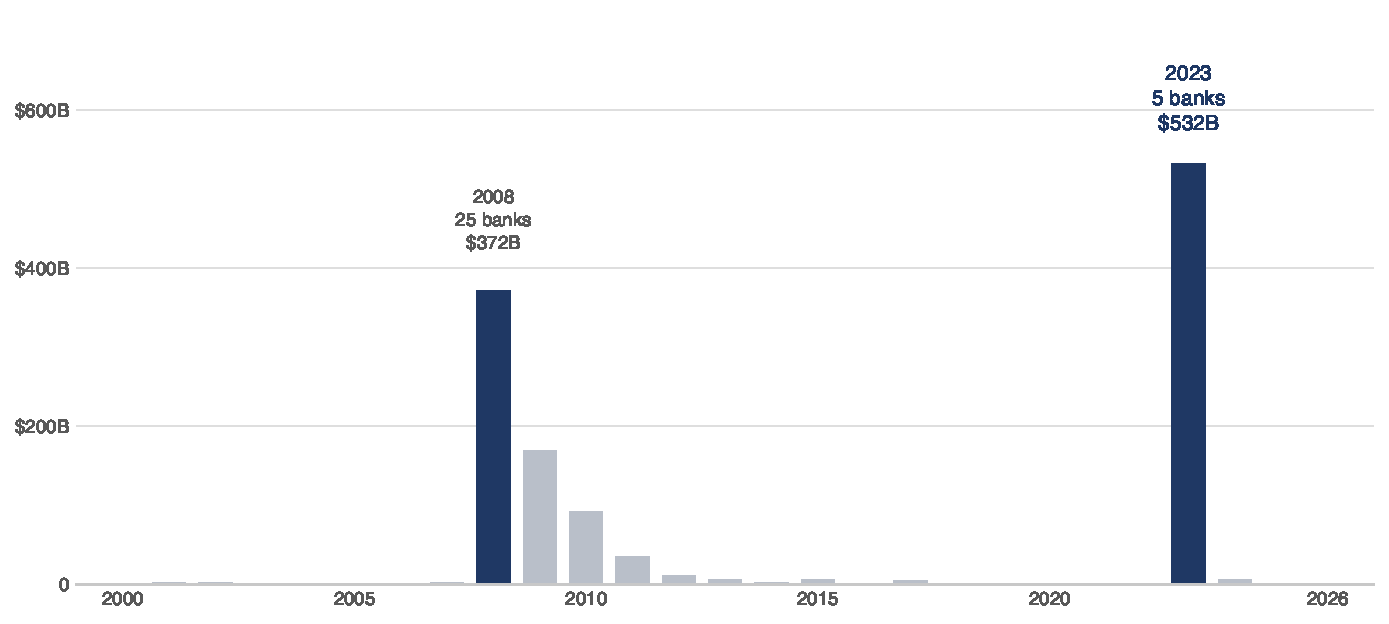
\includegraphics[width=0.92\textwidth]{fail_assets_chart.pdf}\par\vspace{4pt}
  {\sffamily\fontsize{7.5}{10}\selectfont\color{midgray}Total assets of failed U.S. banks by year. Source: FDIC BankFind Failures data (assistance transactions excluded).}
\end{frame}

% ---------- Slide 3: The question and the three blanks ----------
\begin{frame}
  \slidelabel{The question}
  \vspace{4pt}
  {\fontsize{16}{22}\selectfont Which U.S.\ banks are at risk of becoming\\undercapitalized, and how soon?}\par
  \vspace{30pt}
  \begin{columns}[t]
    \begin{column}{0.31\textwidth}
      {\sffamily\bfseries\fontsize{9}{12}\selectfont\color{navy}WHO ACTS}\par\vspace{4pt}
      {\fontsize{10.5}{14}\selectfont The bank's risk department, management, and the board; regulators second.}
    \end{column}
    \begin{column}{0.31\textwidth}
      {\sffamily\bfseries\fontsize{9}{12}\selectfont\color{navy}WHAT THEY DO}\par\vspace{4pt}
      {\fontsize{10.5}{14}\selectfont Raise capital, cut dividends, fix the balance sheet, while the options are still theirs.}
    \end{column}
    \begin{column}{0.31\textwidth}
      {\sffamily\bfseries\fontsize{9}{12}\selectfont\color{navy}IF NOBODY ACTS}\par\vspace{4pt}
      {\fontsize{10.5}{14}\selectfont Mandatory restrictions, then receivership, as happened to SVB in 2023.}
    \end{column}
  \end{columns}
\end{frame}

% ---------- Slide 4: Data + angle ----------
\begin{frame}
  \slidelabel{How, and why me}
  \vspace{2pt}
  \begin{itemize}\itemsep=9pt
    \item {\fontsize{11.5}{15}\selectfont \textbf{Public data:} quarterly FDIC filings for every insured bank since 1992, including the same capital ratios regulators use.}
    \item {\fontsize{11.5}{15}\selectfont \textbf{The model:} flag the banks at risk of becoming undercapitalized, and how soon, before the options run out.}
    \item {\fontsize{11.5}{15}\selectfont \textbf{My angle:} two years at a broker-dealer working with risk and compliance teams; I have seen how these signals get used in practice.}
  \end{itemize}
  \vspace{16pt}
  \textcolor{hairline}{\rule{\textwidth}{0.5pt}}\par\vspace{8pt}
  {\fontsize{12}{16}\selectfont\itshape\color{midgray}Catch the risk while it is still the bank's choice.}
\end{frame}

\end{document}
